\section{Slicing-Algorithmen}

\begin{frame}{Slicing-Algorithmen}
    \begin{description}
        \item[Sphären-Algorithmus] 
        Sphärenförmige Ausbreitung ausgehend von einem Startpunkt.
        \vspace{0.5cm}
        \item[Base-Algorithmus] 
        Planares Slicing entlang einer sich ändernden Normalen.
        \vspace{0.5cm}
        \item[Kristall-Algorithmus] 
        Kombination aus Sphären- und Base-Algorithmus.
    \end{description}
\end{frame}

\begin{frame}{Sphären-Algorithmus}
    \begin{columns}[T]
        % Linke Spalte für den Text
        \begin{column}{0.6\textwidth}
            \begin{itemize}
                \item Ausbreitung in Sphären um einen Startpunkt.
                \vspace{0.5cm}
                \item Wahl eines neuen Startpunkts anhand der Druckernormalen.
            \end{itemize}
        \end{column}

        % Rechte Spalte für das Bild
        \begin{column}{0.4\textwidth}
            \centering
            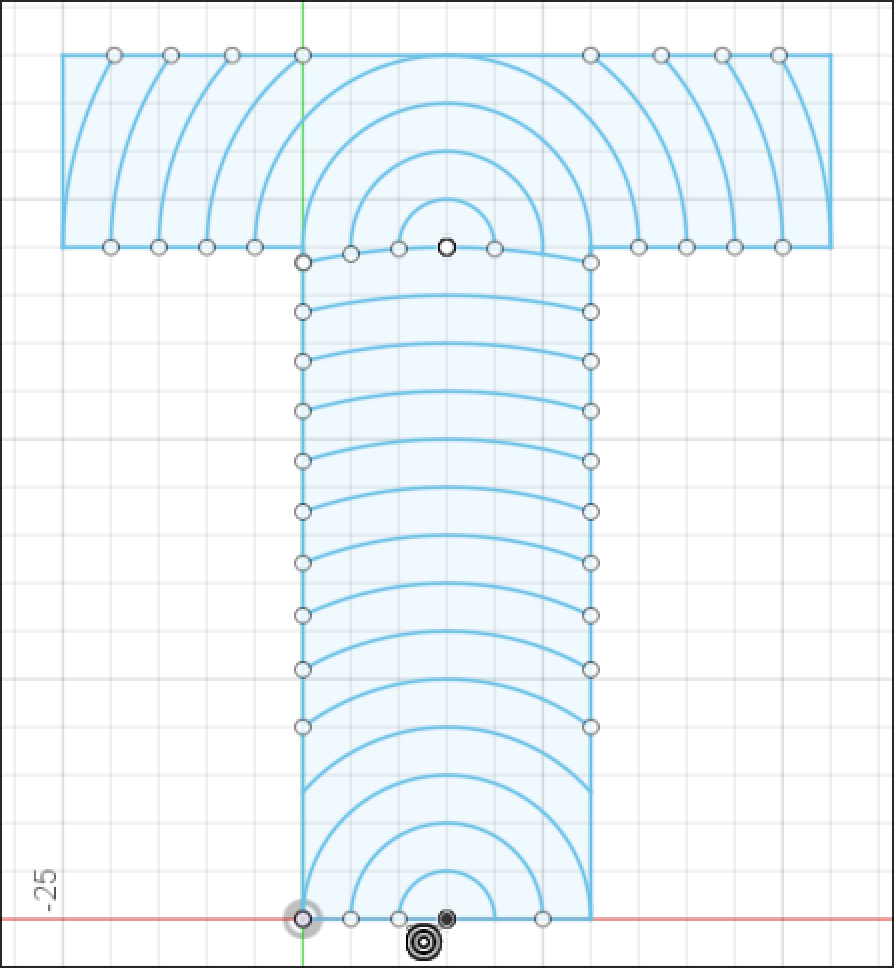
\includegraphics[width=\textwidth]{images/sphere.png}
        \end{column}
    \end{columns}
\end{frame}

\begin{frame}{Base-Algorithmus}
    \begin{columns}[T]
        % Linke Spalte für den Text
        \begin{column}{0.6\textwidth}
            \begin{itemize}
                \item Wahl einer Startnormalen.
                \vspace{0.5cm}
                \item Planares Slicing entlang der Normalen.
                \vspace{0.5cm}
                \item Wahl einer neuen Normalen bei einem Überhang.
            \end{itemize}
        \end{column}

        % Rechte Spalte für das Bild
        \begin{column}{0.4\textwidth}
            \centering
            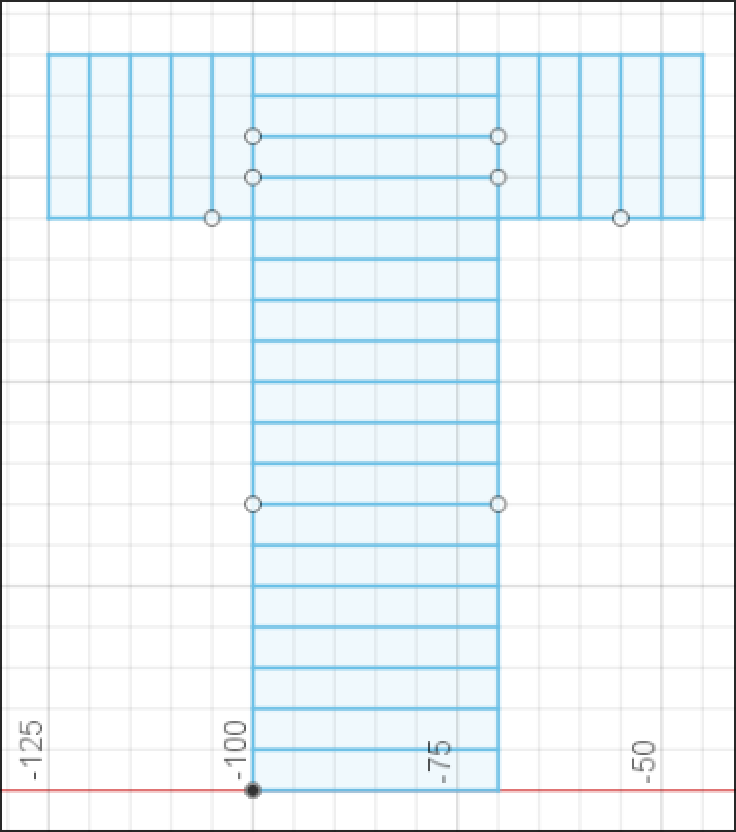
\includegraphics[width=\textwidth]{images/base.png}
        \end{column}
    \end{columns}
\end{frame}

\begin{frame}{Kristall-Algorithmus}
    \begin{columns}[T]
        % Linke Spalte für den Text
        \begin{column}{0.6\textwidth}
            \begin{itemize}
                \item Kombination aus Sphären- und Base-Algorithmus.
                \vspace{0.5cm}
                \item Wahl einer Startnormalen und planares Slicing entlang der Normalen.
                \vspace{0.5cm}
                \item Frühzeitige Erkennung eines Überhanges.
                \vspace{0.5cm}
                \item Langsames Aufbauen einer Sphäre.
            \end{itemize}
        \end{column}

        % Rechte Spalte für das Bild
        \begin{column}{0.4\textwidth}
            \centering
            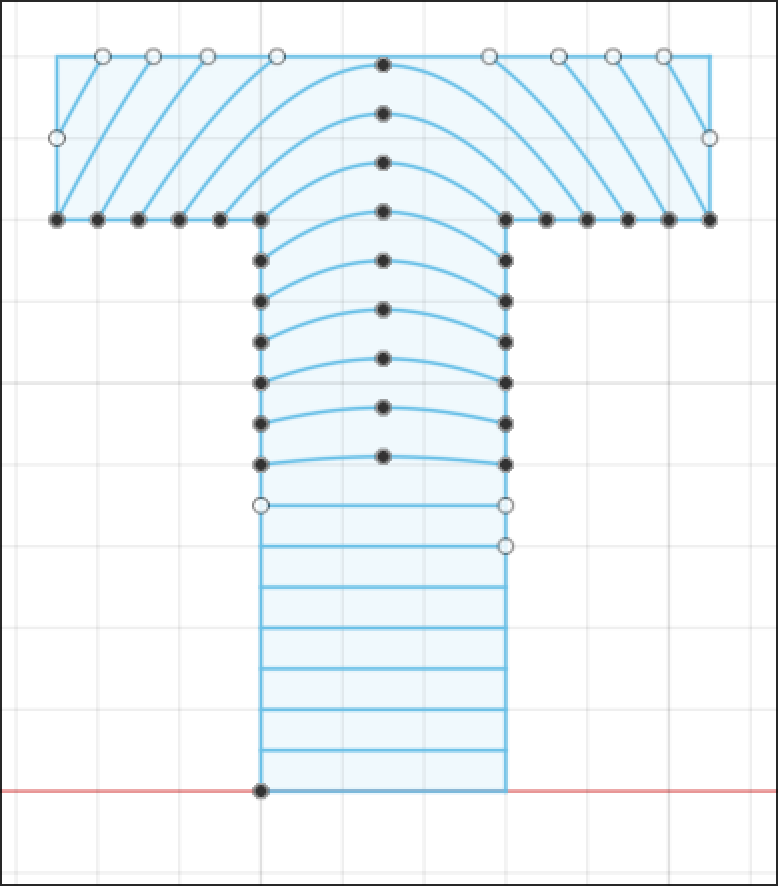
\includegraphics[width=\textwidth]{images/kristall.png}
        \end{column}
    \end{columns}
\end{frame}
